
\section{Deterministic price search and extended simulation benchmarks}\label{supp:note4}

\subsection{Executable price and action updates}
The implementation uses the interval table from Supplementary Note~7 and integer
scores \(H_{es}=\lceil\Gamma\overline q_{es}\rceil\), where \(e=\{i,j\}\),
\(\Gamma=2^{40}\) and \(\overline q\) already subtracts the total-power price.
Write \(F=H/\Gamma\), \(g_{is}=\|h_{is}\|^2\), and
\(r_{es}=|h_{is}^{H}h_{js}|^2/(g_{is}g_{js})\).
The deterministic price is the nearest integer to
\(\operatorname{median}_{i,s}g_{is}/(1+0.1g_{is})\), clipped to \([0,10]\).
Its initial concave-envelope anchor is
\(\operatorname{clip}(1/\max(1,\lambda)-1/G_{is},0.05,0.20)\), with
the positive upper norm endpoint \(G_{is}\) protected against underflow.
For every pair the two highest-scoring tones enter a refinement pool.
At most \(\max(2,\lfloor K^2/32\rfloor)\) pair--tone roots are refined.
The deterministic priority is the priced upper score, and a learned-only run uses
the predicted priority. All roots remain covered.

Define the implemented price quantizer
\[
 {\cal T}(v)=\Gamma^{-1}\operatorname{rint}
 \{\Gamma\operatorname{clip}(v-\overline v,-32,32)\}.
\]
At a price iterate \(\beta\), exact general matching uses
\(w_e=\max_s(H_{es}-\Gamma\beta_s)\).
Bipartite assignment of the resulting matching uses the unpriced \(H\).
Its tone dual potentials, divided by \(\Gamma\) and centred, form \(a\).
The update uses the lowest-bound iterate found within the current branch,
denoted \((\beta_*,M_*)\). For this iterate let
\[
 n_s=\sum_{e\in M_*}{\bf1}
 \{s=\arg\max_t(F_{et}-\beta_{*,t})\}-1,\qquad
 c_s=\tfrac12\sum_i{\bf1}\{s=s_i\}-1 ,
\]
where \((j_i,s_i)\) maximizes \(F_{\{i,j\},s}-\beta_{*,s}-u_j\) over
\(j\ne i,s\), and \(u_j=S^{-1}\sum_s\log(1+0.1g_{js})\).
The next price is
\begin{equation}\label{supp:priceupdate}
 \beta_{\rm next}={\cal T}\!\left[
 0.42\beta_*+0.58a+
 \frac{0.05}{1+0.35\max(0,\ell-2)}
 (0.75n+0.25c)\right].
\end{equation}
Here \(\ell\) starts at zero in each branch. Discrete ties follow the ordered
array operations in the released code. The following steps specify the search.

\begin{enumerate}
\item Build and quantize \(H\). Initialize a nominal matching using the
best equal-power rate of each pair over tones.
\item In the deterministic branch evaluate seven price iterates at \(K\le32\) and six
at \(K=64\). The first three initializers are zero, the centred tone-wise
mean of \(F\), and a centred tone price from assigning users to two duplicate
slots per tone with scores \(\log(1+0.1g_{is})\).
Subsequent iterates use equation~\eqref{supp:priceupdate}.
\item Retain the smallest valid upper objective over the branch. Check its
odd-set witness. On an arithmetic failure, the vertex-price repair supplies
a valid upper witness and the conflict statistic is left undefined.
\item Form feasible candidates from the sequential pairing and all matchings
visited so far. Assign distinct tones using nominal equal-power rates,
then perform up to four sweeps over pairs of assigned tones.
Each sweep considers a tone swap and the four ordered allocations obtained
by exchanging partners between the two pairs.
\item Candidate edges include every incumbent edge and up to
\(\min(6,S)\) disjoint edges per tone selected by a user-centred nominal score.
Accept a local exchange only if both edges are allowed and the score rises
by more than \(10^{-11}\). Deduplicate complete assignments, rank their
nominal rates, and refine the best three.
\item Certify each refined action with its actual powers and receive filters.
Retain the largest checked lower endpoint. In learned warm start, append
three learned-price iterates while preserving the deterministic upper and lower
incumbents. A learned-only run uses one learned-price iterate and one
matched/assigned action.
\end{enumerate}

For fixed assigned partners, let \(x=p_i g_i\), \(y=p_j g_j\) and
\(D=1+x+y+(1-r)xy\). The rate gradient is
\[
 \partial_{p_i}q=g_i\!\left[\frac{2\{1+(1-r)y\}}{D}
                  -\frac{1}{1+x}\right],
\]
with the symmetric expression for \(j\).
Four trial steps use
\(p'=\Pi[p+\eta\,0.05\,\nabla q/\max(10^{-12},\|\nabla q\|_\infty)]\),
\(\eta\in\{1,\tfrac12,\tfrac14,\tfrac18\}\).
Each is accepted only when the nominal sum rate does not decrease.
Here \(\Pi\) is the implemented feasible integer map. With
\(P_T=20\,2^{20}\), first round \(P_Tp_i\) and clip to
\([P_T/20,P_T/5]\). If the sum exceeds \(KP_T/10\), scale each excess
above \(P_T/20\) by \(KP_T/20\) divided by the total excess and round
down. Dividing the final ticks by \(P_T\) gives physical powers.
This map can leave power unused. Separate MMSE combining vectors
are recomputed at the accepted powers before the lower endpoint is checked.

\subsection{Message passing, supervision and the held-out seed choice}
Let \(E=K(K-1)/2\) be the number of pairs.
The network has user, pair, tone and pair--tone factor states of width
\(d=32\). Its seven factor inputs are
\[
 x_{es}=(a_i+a_j,\ |a_i-a_j|,\ r_{es},\
        s/\max(1,S-1),\ 0,\tfrac12,2),\qquad
 a_i=\tfrac15\log(1+0.1g_{is}),
\]
with zero-based tone indices and coordinate zero when \(S=1\). Initial factor states are
\(f^0_{es}=\operatorname{ReLU}(W_xx_{es}+b_x)\).
Initial pair and tone states are their means over tones and pairs.
The initial user state is the mean of its \(K-1\) incident pair states.
Each of three residual layers applies independent two-affine-layer maps
\(\phi(z)=W_2\operatorname{ReLU}(W_1z+b_1)+b_2\), with hidden width 32.
The ordered updates are
\begin{align*}
 f^{\ell+1}_{es}&=f^\ell_{es}+
 \phi_f^\ell([f^\ell_{es},e^\ell_e,t^\ell_s,
                         u^\ell_i+u^\ell_j,|u^\ell_i-u^\ell_j|]),\\
 e^{\ell+1}_e&=e^\ell_e+
 \phi_e^\ell([e^\ell_e,S^{-1}\textstyle\sum_s f^{\ell+1}_{es}]),\\
 t^{\ell+1}_s&=t^\ell_s+
 \phi_t^\ell([t^\ell_s,E^{-1}\textstyle\sum_e f^{\ell+1}_{es}]),\\
 u^{\ell+1}_i&=u^\ell_i+
 \phi_u^\ell([u^\ell_i,(K-1)^{-1}\textstyle\sum_{e\ni i}e^{\ell+1}_e]).
\end{align*}
Thus pair permutation and user exchange are respected by the shared maps,
while tone position is explicitly present in the input.

Two user outputs give \(p_i=0.05+0.15\sigma(z_{i1})\) and the centred
\(\alpha_i=z_{i2}-K^{-1}\sum_jz_{j2}\).
A tone head gives centred \(\beta_s\), a global mean-user head gives
\(\lambda=12\sigma(z_\lambda)\), and a factor head adds a residual
\(0.1z_{es}\) to the observed equal-power pair rate.
A shared box head reads \([f_{es},l_1,u_1,l_2,u_2]\) in normalized box
coordinates and returns two sigmoid-mapped anchors in \([0.05,0.20]\)
and one unconstrained priority. The same head scores root boxes and
the two half-boxes used in priority supervision. At inference the worker
evaluates both half-boxes for the \(\max(2,\lfloor K^2/32\rfloor)\)
highest-priority factors and adds \(0.05\) times the larger child score
to each selected root priority. Pair-endpoint anchor suggestions are
averaged over the \(K-1\) incident pairs to produce each user's anchor
on a tone. GPU timing includes these head evaluations and aggregation.
There are 52,776 trainable
parameters. The hybrid search consumes the predicted tone prices
while retaining the deterministic power-price/enclosure table and its deterministic
action pool. The network-only comparator additionally uses the predicted
power price, anchors, priorities, pair scores and powers.
The predicted user-price head is supervised but is not used by the
deterministic solver's upper certificate.

Teachers were generated on 4,096 fitting blocks only, comprising 1,024
blocks from each of the analytic, CDL-A, CDL-B and CDL-C generators.
User counts were \(8,16,32\), with \(1,368,1,364,1,364\) examples,
respectively. SNRs were \(0,10,20\) dB. The teacher solver produced
feasible actions, power-price and dual targets, enclosure anchors, 57,296
visited-root labels and 56,571 strict sibling-priority comparisons.
The median teacher interval was 0.083914 bit/s/Hz and median recorded
teacher time was 9.487 ms. Before this training run, tone-price targets
were recomputed from an exact assignment of equal-power nominal scores
for the teacher's selected pairs.

The loss sums an equally positive/negative-weighted logistic pair-assignment
loss, mean-square power and anchor errors divided by \(0.15^2\), centred
user/tone-price errors divided by \(4^2\), power-price error divided by
\(10^2\), and softplus ranking losses for strict sibling and visited-root
priority comparisons. Priority pairs whose target difference is at most
\(10^{-10}\) are omitted. Batches have at most eight examples of one size.
Each of seeds 1729, 2718 and 3141 receives 15 epochs over all 4,096 examples,
7,695 Adam updates at learning rate \(10^{-3}\), and gradient-norm clipping
at 3. TensorFloat-32 matrix products are disabled.
The recorded GPU was an NVIDIA Quadro RTX 4000 with Max-Q Design.

Seed selection uses 256 separate validation blocks and the mean empirical
coverage of gap cutoffs \(0.02\), \(0.05\), \(0.10\) and \(0.15\) bit/s/Hz. Ties are broken
by median gap, median latency, then seed. Seed 1729 was locked before
the primary test. Supplementary Table~\ref{supp:table4} also gives component swaps on a
separate post-freeze benchmark of all 512 native 32-user blocks.
Those swaps retain the deterministic power price and replace the named
field. Their baseline is rerun within that benchmark.

The original learned-versus-deterministic pass increases were 1.17 percentage points at 32 users (95\% stratified bootstrap interval 0.39--2.15) and 0.98 at 64 users (0.20--1.95). The original resource-subgradient baseline passed on 359 of 512 and 294 of 512 topologies, respectively, with a median complete time of 715 ms at 64 users.

\subsection{Timing cohorts, sensitivity records and the selectivity diagnostic}
Supplementary Table~\ref{supp:table3} and Supplementary Fig.~\ref{supp:fig1} use the 12,288 timed
primary calls. For each topology and method, the primary gap is the
largest of three returned gaps and latency is the median of three
complete calls. A pass requires \(G\le0.15\) bit/s/Hz and median time
at most 250 ms for 32 users or 1,000 ms for 64 users.
There are 128 independent blocks per profile. Timers start after channel
cropping and normalization, with kernels and the GPU worker already warmed.
Stage summaries first take
the median of the three stage times within each block, then the indicated
quantile over blocks. Host neural time includes the prediction request
and response. GPU time is the worker's synchronized forward measurement
and overlaps host neural time. It is not an additional stage to sum.
Serialization and other orchestration are included in complete time.
Medians of separate stages need not add to the median complete time.

The separate shuffled-order experiment draws 52 blocks by a fixed hash
ranking and makes one additional call per size and method in permuted
method order (416 calls). Supplementary Fig.~\ref{supp:fig2} compares each such time
with the same block's original median. These data describe load/order
sensitivity and do not replace the primary deadline decisions.

The sensitivity grid contains 13,824 deterministic cells
\((6,144\ {\rm native},6,144\ {\rm analytic},1,536\ {\rm ray})\),
covering four SNRs, three user counts and 1,152 base topologies.
Three classical controls are evaluated on every cell.
The network-only, learned-warm-start and subgradient-baseline controls use a shared learned
proposal in 12,800 non-primary cells. Their recorded component times include
the shared proposal's time and cannot be substituted for complete primary
timings. The remaining 1,024 native 10-dB cells use the three-repeat
primary records for those methods. The full 96,768 method-cell records
and all family/size/SNR/method summaries are archived in the repository for
Supplementary Table~\ref{supp:table5}. Classical control runs use the same native
matching implementation as the deterministic solver, whereas the primary
subgradient baseline retains its original matching implementation.
No timing cohorts are pooled for a new pass/fail claim.

The fixed-policy selectivity experiment uses 128 analytic 16-user channels
interpolated at nine values between the first-tone channel and the
frequency-selective channel. At each interpolation the sequential pairing,
tone order and 0.10-W powers are fixed, with its receiver recomputed for
that input. Its interval ranges from 0.035915 to 2.343011 bit/s/Hz.
The ratio of the \emph{price-selected matching's} conflict bound to this
fixed action's interval never exceeds 0.377035.
However, the actual fixed-action decomposition \(T_2\) exceeds half the interval
in 980 of 1,152 cases. The two numerators belong to different pairings,
as shown in Supplementary Fig.~\ref{supp:fig3}.
For the separate optimized native primary cohort, mean \(T_2\) is
0.041201 of a 0.065232-bit/s/Hz mean interval at 32 users and
0.058741 of 0.072248 at 64 users. These observations do not identify a
universal transition of optimized schedules from the frozen-action
crossing test. Supplementary Fig.~\ref{supp:fig4} tests the posterior bound against
the exact optimum of the same rounded table at 16 users, separately
within each native profile.


\begingroup\small\setlength{\tabcolsep}{4pt}
\begin{longtable}{lrlrrrr}\caption{Native 10-dB primary results by profile. Panel A gives gap quantiles (bit/s/Hz) and joint passes; Panel B gives median stage times (ms). GPU time is included in host prediction time.}\label{supp:table3}\\
\toprule Method & $K$ & Profile & Pass & p05 & p50 & p95\\\midrule\endfirsthead\toprule Method & $K$ & Profile & Pass & p05 & p50 & p95\\\midrule\endhead\bottomrule\endfoot
Subgradient baseline & 32 & A & 101/128 & 0.071 & 0.121 & 0.179\\
Deterministic search & 32 & A & 126/128 & 0.037 & 0.077 & 0.117\\
Network only & 32 & A & 74/128 & 0.088 & 0.145 & 0.198\\
Learned warm start & 32 & A & 128/128 & 0.030 & 0.070 & 0.110\\
Subgradient baseline & 32 & B & 119/128 & 0.059 & 0.102 & 0.145\\
Deterministic search & 32 & B & 128/128 & 0.022 & 0.055 & 0.091\\
Network only & 32 & B & 104/128 & 0.074 & 0.119 & 0.186\\
Learned warm start & 32 & B & 128/128 & 0.017 & 0.051 & 0.085\\
Subgradient baseline & 32 & C & 127/128 & 0.040 & 0.079 & 0.117\\
Deterministic search & 32 & C & 128/128 & 0.024 & 0.050 & 0.078\\
Network only & 32 & C & 125/128 & 0.059 & 0.095 & 0.146\\
Learned warm start & 32 & C & 128/128 & 0.023 & 0.046 & 0.073\\
Subgradient baseline & 32 & UMa & 12/128 & 0.113 & 0.205 & 0.377\\
Deterministic search & 32 & UMa & 124/128 & 0.008 & 0.074 & 0.139\\
Network only & 32 & UMa & 0/128 & 0.270 & 0.399 & 0.552\\
Learned warm start & 32 & UMa & 128/128 & 0.003 & 0.062 & 0.129\\
Subgradient baseline & 64 & A & 97/128 & 0.084 & 0.121 & 0.162\\
Deterministic search & 64 & A & 128/128 & 0.046 & 0.084 & 0.109\\
Network only & 64 & A & 85/128 & 0.103 & 0.139 & 0.182\\
Learned warm start & 64 & A & 128/128 & 0.046 & 0.078 & 0.098\\
Subgradient baseline & 64 & B & 96/128 & 0.065 & 0.093 & 0.130\\
Deterministic search & 64 & B & 128/128 & 0.032 & 0.053 & 0.073\\
Network only & 64 & B & 127/128 & 0.079 & 0.109 & 0.138\\
Learned warm start & 64 & B & 128/128 & 0.031 & 0.050 & 0.073\\
Subgradient baseline & 64 & C & 98/128 & 0.059 & 0.081 & 0.113\\
Deterministic search & 64 & C & 128/128 & 0.040 & 0.055 & 0.077\\
Network only & 64 & C & 128/128 & 0.073 & 0.097 & 0.123\\
Learned warm start & 64 & C & 128/128 & 0.038 & 0.054 & 0.075\\
Subgradient baseline & 64 & UMa & 3/128 & 0.129 & 0.192 & 0.263\\
Deterministic search & 64 & UMa & 120/128 & 0.043 & 0.098 & 0.153\\
Network only & 64 & UMa & 0/128 & 0.310 & 0.379 & 0.473\\
Learned warm start & 64 & UMa & 125/128 & 0.040 & 0.092 & 0.144\\\end{longtable}\addtocounter{table}{-1}\renewcommand{\theHtable}{\arabic{table}B}\begin{longtable}{lrlrrrrrr}\multicolumn{9}{l}{\textbf{B. Median stage and complete times}}\\\toprule Method & $K$ & Profile & Box & Dual & Primal & NN & GPU & All\\\midrule\endfirsthead\toprule Method & $K$ & Profile & Box & Dual & Primal & NN & GPU & All\\\midrule\endhead\bottomrule\endfoot
Subgradient baseline & 32 & A & 8.3 & 27.6 & 2.3 & 0.0 & 0.0 & 36.7\\
Deterministic search & 32 & A & 6.5 & 5.9 & 4.3 & 0.0 & 0.0 & 17.8\\
Network only & 32 & A & 7.2 & 1.4 & 0.8 & 16.8 & 11.9 & 27.1\\
Learned warm start & 32 & A & 6.4 & 8.8 & 9.6 & 16.3 & 11.9 & 42.0\\
Subgradient baseline & 32 & B & 8.2 & 51.0 & 2.5 & 0.0 & 0.0 & 72.4\\
Deterministic search & 32 & B & 6.3 & 5.9 & 4.3 & 0.0 & 0.0 & 17.3\\
Network only & 32 & B & 7.1 & 1.5 & 0.8 & 16.0 & 11.4 & 26.3\\
Learned warm start & 32 & B & 6.4 & 9.1 & 9.5 & 16.0 & 11.4 & 41.6\\
Subgradient baseline & 32 & C & 8.2 & 27.6 & 2.5 & 0.0 & 0.0 & 38.2\\
Deterministic search & 32 & C & 6.4 & 5.8 & 4.3 & 0.0 & 0.0 & 17.8\\
Network only & 32 & C & 7.2 & 1.4 & 0.8 & 17.8 & 12.2 & 28.0\\
Learned warm start & 32 & C & 6.4 & 9.1 & 9.4 & 17.8 & 12.1 & 42.7\\
Subgradient baseline & 32 & UMa & 8.4 & 88.6 & 35.5 & 0.0 & 0.0 & 136.7\\
Deterministic search & 32 & UMa & 6.6 & 6.8 & 4.4 & 0.0 & 0.0 & 18.9\\
Network only & 32 & UMa & 7.3 & 1.8 & 0.8 & 17.5 & 12.2 & 27.6\\
Learned warm start & 32 & UMa & 6.6 & 10.5 & 9.5 & 17.0 & 11.9 & 44.3\\
Subgradient baseline & 64 & A & 61.4 & 214.4 & 4.3 & 0.0 & 0.0 & 324.4\\
Deterministic search & 64 & A & 50.2 & 13.5 & 9.4 & 0.0 & 0.0 & 76.2\\
Network only & 64 & A & 55.2 & 3.8 & 1.1 & 78.2 & 63.1 & 142.2\\
Learned warm start & 64 & A & 50.4 & 22.0 & 20.3 & 78.2 & 63.0 & 174.3\\
Subgradient baseline & 64 & B & 60.8 & 428.9 & 193.8 & 0.0 & 0.0 & 720.9\\
Deterministic search & 64 & B & 49.8 & 14.0 & 9.3 & 0.0 & 0.0 & 75.9\\
Network only & 64 & B & 55.2 & 3.9 & 1.1 & 78.6 & 63.1 & 142.6\\
Learned warm start & 64 & B & 49.3 & 22.0 & 20.4 & 77.8 & 63.0 & 172.8\\
Subgradient baseline & 64 & C & 62.4 & 421.8 & 89.9 & 0.0 & 0.0 & 559.4\\
Deterministic search & 64 & C & 52.1 & 15.1 & 9.5 & 0.0 & 0.0 & 80.7\\
Network only & 64 & C & 55.7 & 3.9 & 1.0 & 78.0 & 63.1 & 142.5\\
Learned warm start & 64 & C & 49.4 & 24.6 & 19.7 & 78.1 & 63.0 & 175.4\\
Subgradient baseline & 64 & UMa & 62.2 & 969.9 & 325.6 & 0.0 & 0.0 & 1354.2\\
Deterministic search & 64 & UMa & 50.5 & 19.3 & 9.3 & 0.0 & 0.0 & 82.2\\
Network only & 64 & UMa & 55.6 & 5.1 & 1.1 & 78.9 & 63.2 & 144.5\\
Learned warm start & 64 & UMa & 50.1 & 30.4 & 19.8 & 78.8 & 63.1 & 184.0\\\end{longtable}\endgroup
\begin{table}[htbp]\centering\small
\caption{Frozen seed selection and post-freeze component swaps. Validation scores average four gap cutoffs fixed before test evaluation. Swap values are median gaps in bit/s/Hz at 32 users and 10 dB, with 128 blocks per profile.}\label{supp:table4}
\begin{tabular}{rrrrrr}\toprule Seed & Score & Median gap & Median ms & Final loss & Train s\\\midrule
1729* & 0.774414 & 0.026817 & 26.14 & 0.5283 & 321.8\\
2718 & 0.769531 & 0.029212 & 27.15 & 0.5261 & 358.9\\
3141 & 0.766602 & 0.029347 & 23.19 & 0.5625 & 375.3\\
\bottomrule\end{tabular}\par\smallskip
\begin{tabular}{lrrrr}\toprule Component setting & CDL-A & CDL-B & CDL-C & UMa\\\midrule
Deterministic baseline & 0.076966 & 0.055182 & 0.049558 & 0.073799\\
Learned tone price & 0.097881 & 0.073606 & 0.061210 & 0.134411\\
Learned primal proposal & 0.110202 & 0.092150 & 0.071688 & 0.233375\\
Learned enclosure anchor & 0.088209 & 0.066604 & 0.059210 & 0.176799\\
Learned refinement priority & 0.076966 & 0.055182 & 0.049558 & 0.073800\\
Vertex-price repair & 0.205371 & 0.145467 & 0.164225 & 0.742815\\
One-hidden-layer MLP & 0.869022 & 0.753858 & 0.489869 & 1.895399\\
\bottomrule\end{tabular}\par\smallskip\footnotesize *Selected before testing. The MLP has 32 hidden units and five fitting passes. Its inputs are matched to the pair features used by the message-passing model.\end{table}
\begin{table}[htbp]\centering\small
\setlength{\tabcolsep}{3pt}
\caption{Sensitivity-grid summary. Each entry is a median certified gap in bit/s/Hz over 512 native, 512 analytic or 128 ray-traced topologies at the indicated size and SNR. Zero denotes the zero-price baseline, Match the equal-power-initialized matching with power refinement control and Seq. sequential pairing. Full per-family quantiles and seven-method comparisons are available in the repository CSV files.}\label{supp:table5}
\begin{tabular}{lllllll}\toprule
Campaign & $K$ & SNR (dB) & Deterministic search & Zero & Match & Seq.\\\midrule
native & 16 & -5 & 0.047 & 0.325 & 1.897 & 2.609\\
native & 16 & 0 & 0.035 & 0.396 & 2.059 & 2.899\\
native & 16 & 10 & 0.024 & 0.503 & 2.138 & 3.050\\
native & 16 & 20 & 0.025 & 0.499 & 2.146 & 3.067\\
native & 32 & -5 & 0.073 & 0.318 & 1.924 & 2.757\\
native & 32 & 0 & 0.066 & 0.401 & 2.075 & 3.059\\
native & 32 & 10 & 0.061 & 0.513 & 2.146 & 3.219\\
native & 32 & 20 & 0.061 & 0.510 & 2.153 & 3.236\\
native & 64 & -5 & 0.077 & 0.291 & 1.912 & 2.813\\
native & 64 & 0 & 0.073 & 0.373 & 2.055 & 3.117\\
native & 64 & 10 & 0.067 & 0.488 & 2.122 & 3.284\\
native & 64 & 20 & 0.067 & 0.485 & 2.129 & 3.303\\
analytic & 16 & -5 & 0.014 & 0.234 & 1.797 & 2.094\\
analytic & 16 & 0 & 0.007 & 0.276 & 1.938 & 2.301\\
analytic & 16 & 10 & 0.001 & 0.370 & 2.002 & 2.402\\
analytic & 16 & 20 & 0.000 & 0.365 & 2.000 & 2.413\\
analytic & 32 & -5 & 0.014 & 0.222 & 1.799 & 2.068\\
analytic & 32 & 0 & 0.010 & 0.280 & 1.945 & 2.358\\
analytic & 32 & 10 & 0.002 & 0.382 & 2.013 & 2.479\\
analytic & 32 & 20 & 0.002 & 0.377 & 2.020 & 2.491\\
analytic & 64 & -5 & 0.014 & 0.214 & 1.790 & 2.061\\
analytic & 64 & 0 & 0.010 & 0.267 & 1.934 & 2.356\\
analytic & 64 & 10 & 0.003 & 0.370 & 2.002 & 2.535\\
analytic & 64 & 20 & 0.003 & 0.369 & 2.013 & 2.547\\
ray & 16 & -5 & 0.374 & 0.677 & 1.852 & 2.551\\
ray & 16 & 0 & 0.384 & 0.853 & 2.055 & 3.300\\
ray & 16 & 10 & 0.246 & 0.831 & 2.250 & 4.082\\
ray & 16 & 20 & 0.120 & 0.700 & 2.222 & 4.304\\
ray & 32 & -5 & 0.360 & 0.568 & 1.826 & 2.716\\
ray & 32 & 0 & 0.355 & 0.757 & 2.022 & 3.597\\
ray & 32 & 10 & 0.221 & 0.754 & 2.215 & 4.389\\
ray & 32 & 20 & 0.111 & 0.660 & 2.203 & 4.778\\
ray & 64 & -5 & 0.387 & 0.552 & 1.836 & 2.752\\
ray & 64 & 0 & 0.392 & 0.752 & 2.029 & 3.673\\
ray & 64 & 10 & 0.208 & 0.747 & 2.203 & 4.599\\
ray & 64 & 20 & 0.134 & 0.648 & 2.180 & 4.790\\
\bottomrule\end{tabular}\end{table}

\begin{table}[htbp]\centering\small
\setlength{\tabcolsep}{4pt}
\caption{Native rates at 10 dB on 512 topologies per size. Rates are medians in bit/s/Hz. $U_{\rm best}$ is the smallest verified ceiling across all seven methods on the same topology. Retention is the median of $100 L/U_{\rm best}$. Across repeated calls each endpoint minimum is taken separately.}\label{supp:rates}
\begin{tabular}{llllll}\toprule
$K$ & Method & $L$ & $U$ & $U_{\rm best}$ & Retained (\%)\\
\midrule
16 & Zero-price baseline & 15.1362 & 15.6304 & 15.2188 & 99.451\\
16 & Deterministic search & 15.1928 & 15.2290 & 15.2188 & 99.879\\
16 & Matching + power refinement & 15.1362 & 17.2669 & 15.2188 & 99.451\\
16 & Learned warm start & 15.1964 & 15.2255 & 15.2188 & 99.900\\
16 & Subgradient baseline & 15.1362 & 15.2302 & 15.2188 & 99.451\\
16 & Sequential equal-power & 14.3612 & 17.2669 & 15.2188 & 93.426\\
16 & Network only & 15.1529 & 15.2529 & 15.2188 & 99.461\\
32 & Zero-price baseline & 15.2885 & 15.7868 & 15.3808 & 99.322\\
32 & Deterministic search & 15.3312 & 15.3881 & 15.3808 & 99.636\\
32 & Matching + power refinement & 15.2885 & 17.4203 & 15.3808 & 99.322\\
32 & Learned warm start & 15.3356 & 15.3857 & 15.3808 & 99.675\\
32 & Subgradient baseline & 15.2885 & 15.3875 & 15.3808 & 99.322\\
32 & Sequential equal-power & 14.3288 & 17.4203 & 15.3808 & 92.320\\
32 & Network only & 15.2969 & 15.4171 & 15.3808 & 99.348\\
64 & Zero-price baseline & 15.4007 & 15.8814 & 15.4897 & 99.392\\
64 & Deterministic search & 15.4301 & 15.4897 & 15.4897 & 99.587\\
64 & Matching + power refinement & 15.4007 & 17.5153 & 15.4897 & 99.392\\
64 & Learned warm start & 15.4311 & 15.4897 & 15.4897 & 99.601\\
64 & Subgradient baseline & 15.4007 & 15.5035 & 15.4897 & 99.392\\
64 & Sequential equal-power & 14.3363 & 17.5153 & 15.4897 & 91.784\\
64 & Network only & 15.4015 & 15.5230 & 15.4897 & 99.388\\
\bottomrule\end{tabular}
\par\medskip\begin{minipage}{\linewidth}\small
The three matching controls share the same starting pairs and four power-refinement steps. They give identical lower endpoints on each topology. Sequential equal-power uses 0.10 W per user. At 16, 32 and 64 users, the zero-price decision meets the 0.15-bit/s/Hz gap on 0, 0 and 0 of 512 topologies using its own ceiling, and on 408, 395 and 426 using the common ceiling. These paired comparisons use rate alone. At 32 and 64 users, the median sums of seven representative call times were 208.45 and 1,429.72 ms. Summing all 15 archived calls gave medians of 539.58 and 3,732.28 ms. Source Data gives the counts by profile and both timing sums for each topology.
\end{minipage}
\end{table}

\begin{table}[htbp]\centering\small
\setlength{\tabcolsep}{4pt}
\caption{Paired iteration- and time-budget controls. Passes require the original gap and deadline criteria. The original confirmatory campaign is unchanged.}\label{supp:compute}
\begin{tabular}{llllll}\toprule
$K$ & Method & Iterations & Passes & Median $G$ & Median ms\\
\midrule
\multicolumn{6}{l}{\textit{Iteration run}}\\
32 & Deterministic search & 7 & 506/512 & 0.06134 & 16.88\\
32 & Equal-iteration deterministic & 10 & 507/512 & 0.05942 & 19.46\\
32 & Learned warm start & 10 & 512/512 & 0.05495 & 39.66\\
64 & Deterministic search & 6 & 504/512 & 0.06662 & 74.02\\
64 & Equal-iteration deterministic & 9 & 505/512 & 0.06612 & 80.81\\
64 & Learned warm start & 9 & 509/512 & 0.06447 & 169.51\\
\multicolumn{6}{l}{\textit{Time-budget run}}\\
32 & Learned warm start & 10 & 512/512 & 0.05495 & 35.59\\
32 & Time-budget deterministic & 38 & 507/512 & 0.05783 & 38.39\\
64 & Learned warm start & 9 & 509/512 & 0.06447 & 164.01\\
64 & Time-budget deterministic & 63 & 505/512 & 0.06318 & 176.35\\
\bottomrule\end{tabular}
\par\medskip\begin{minipage}{\linewidth}\small
\par\smallskip\noindent\begin{tabular}{llrrrrr}\toprule Control & $K$ & Both & Control only & Learned only & Neither & Exact $P$\\\midrule
Iteration & 32 & 507 & 0 & 5 & 0 & 0.0625\\
Iteration & 64 & 505 & 0 & 4 & 3 & 0.125\\
Time budget & 32 & 507 & 0 & 5 & 0 & 0.0625\\
Time budget & 64 & 505 & 0 & 4 & 3 & 0.125\\
\bottomrule\end{tabular}\par\smallskip
Each campaign uses the same 512 topologies, three repeats and rotating method order. A topology uses its largest gap and median time. The iteration control adds three deterministic price updates. For the time-budget control, 16 hash-selected topologies calibrate only timing; the resulting 38/63 deterministic iterations are frozen before the full comparison. The control shares the original power table, update rule and candidate construction. No network is retrained. Absolute times differ between campaigns; matching their medians does not impose equal time on each topology. Exact two-sided McNemar tests condition on discordant topology pairs. All rates are bit/s/Hz.
\end{minipage}
\end{table}

\begin{table}[htbp]\centering\small
\setlength{\tabcolsep}{4pt}
\caption{Ceiling slack and action suboptimality. For a physical reference $V^*\in[V_-,V_+]$, contributions lie in $[U-V_+,U-V_-]$ and $[V_--L,V_+-L]$. Means, medians and endpoint quartiles are reported separately.}\label{supp:decomposition}
\begin{tabular}{lllll}\toprule
$K$ & Channel / reference & Statistic & Ceiling slack & Action suboptimality\\
\midrule
2 & Analytic / roots & Mean & [0.23467, 0.23467] & [0.00340, 0.00340]\\
 &  & 25th percentile & [0.00006, 0.00006] & [1.3e-11, 1.3e-11]\\
 &  & Median & [0.00221, 0.00221] & [1.1e-06, 1.1e-06]\\
 &  & 75th percentile & [0.13947, 0.13947] & [1.1e-05, 1.1e-05]\\
4 & Analytic / 192 splits & Mean & [0.12743, 0.21416] & [0.00110, 0.08783]\\
 &  & 25th percentile & [0.00007, 0.00011] & [0.00000, 5e-05]\\
 &  & Median & [0.00118, 0.00123] & [0.00000, 0.00006]\\
 &  & 75th percentile & [0.10351, 0.13480] & [1.8e-15, 0.03136]\\
6 & Analytic / 192 splits & Mean & [0.05487, 0.20326] & [0.00134, 0.14973]\\
 &  & 25th percentile & [0.00005, 0.00012] & [0.00000, 0.00006]\\
 &  & Median & [0.00081, 0.00090] & [0.00000, 0.00007]\\
 &  & 75th percentile & [0.08775, 0.16254] & [0.00000, 0.12917]\\
8 & Analytic / 192 splits & Mean & [0.03387, 0.20021] & [0.00477, 0.17110]\\
 &  & 25th percentile & [1.5e-09, 0.00016] & [0.00000, 0.00006]\\
 &  & Median & [0.00010, 0.00078] & [0.00000, 0.00037]\\
 &  & 75th percentile & [0.05753, 0.13957] & [0.00000, 0.12273]\\
\bottomrule\end{tabular}
\par\medskip\begin{minipage}{\linewidth}\small
\par\smallskip\noindent\begin{tabular}{llrr}\toprule Family / reference & Statistic & Slack above table & Shortfall below table\\\midrule
Native 3GPP / exact DP & Mean & 0.01756 & 0.01517\\
 & 25th percentile & 0.00482 & 0.00109\\
 & Median & 0.01481 & 0.00389\\
 & 75th percentile & 0.02518 & 0.02214\\
\bottomrule\end{tabular}\par\smallskip
For $K=2$, rational polynomial-root isolation encloses the physical optimum. At $K=4,6,8$, continuous box references allow 192 splits and remain unresolved at $10^{-6}$ bit/s/Hz. Quartiles and medians summarize each bracket endpoint separately; the 25th--75th percentile rows describe their IQRs. At $K=16$, exact integer DP optimizes the upper-score table, giving $V_{\rm tab}\geq V^*$; the displayed $U-V_{\rm tab}$ and $V_{\rm tab}-L$ are an algebraic table-reference split, not physical slack and action loss. No trend across these different channel families is implied. All entries use 512 topologies per size and bit/s/Hz. Reference widths (median; maximum) for $K=2$: 5.32907e-15; 8.88178e-15, $K=4$: 5.85335e-05; 0.514074, $K=6$: 7.33722e-05; 0.854413, $K=8$: 0.000150431; 0.929094.

\end{minipage}
\end{table}

\begin{figure}[htbp]\centering
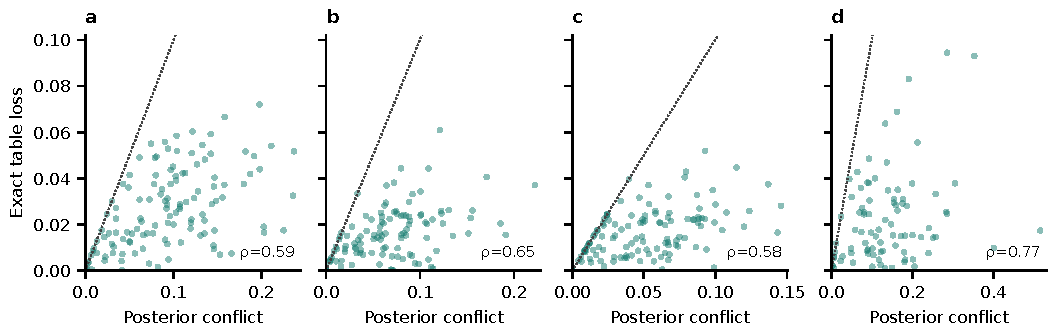
\includegraphics[width=\linewidth]{supplementary/figures/sfig1.pdf}
\caption{Exact labelled-table comparisons at 16 users and 10 dB. Panels a--d show CDL-A, CDL-B, CDL-C and UMa, respectively. Each panel shows 128 independent native blocks. Both axes are in bit/s/Hz. The vertical value is \(R_\beta-D(H)\), and the horizontal value is \(R_\beta-A_\beta\). The dotted diagonal is equality, and each annotation reports its within-profile Spearman correlation. The comparison concerns the rounded integer table.}\label{supp:fig4}
\end{figure}
\begin{figure}[htbp]\centering
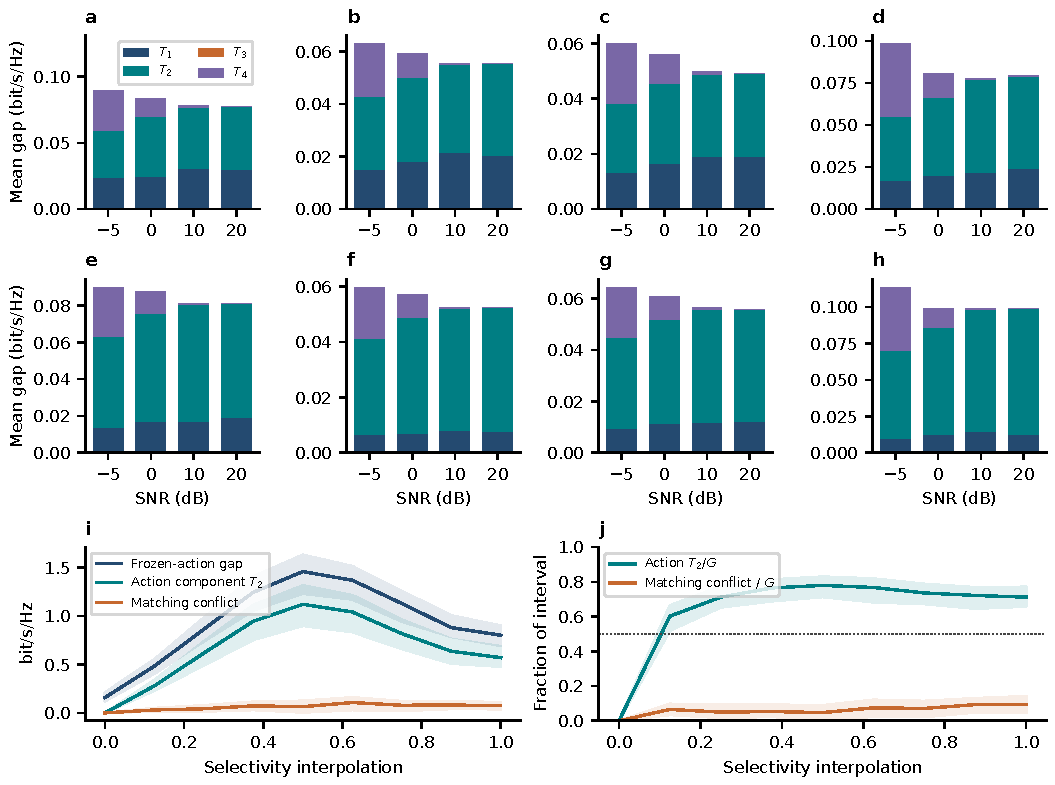
\includegraphics[width=\linewidth]{supplementary/figures/sfig2.pdf}
\caption{Four-term decomposition and the fixed-policy selectivity test. Panels a--d show 32 users and e--h show 64 users, with CDL-A, CDL-B, CDL-C and UMa from left to right. Panels i and j show absolute and relative contributions for the fixed sequential action at 16 users. The upper eight panels stack mean terms over 128 native blocks per profile, size and SNR in the separately timed sensitivity grid. All four means sum to the mean interval, including the small unused-power term. The lower panels show medians and interquartile bands over 128 analytic 16-user blocks at each interpolation. The sequential action's \(T_2\) and the price-selected matching's conflict statistic use different pairings. The dotted line marks one half of the action interval.}\label{supp:fig3}
\end{figure}
\begin{figure}[htbp]\centering
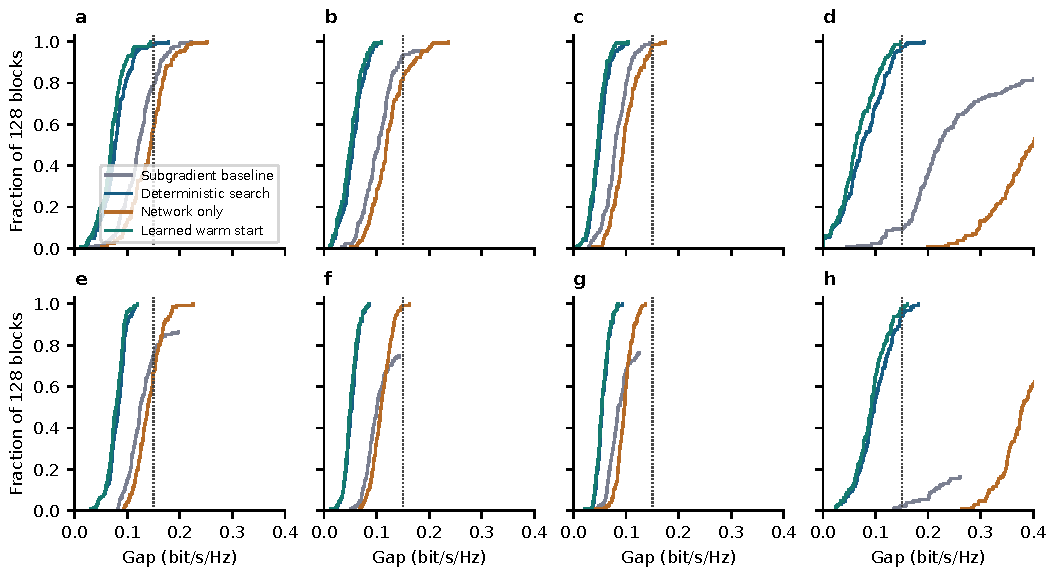
\includegraphics[width=\linewidth]{supplementary/figures/sfig3.pdf}
\caption{Deadline-aware empirical gap distributions within each native profile. Panels a--d show 32 users and e--h show 64 users; within each row the profiles are CDL-A, CDL-B, CDL-C and UMa. Each panel contains 128 independent blocks. Only on-time outcomes increment the curve, and the denominator remains 128. The vertical line is the 0.15-bit/s/Hz criterion. The horizontal display ends at 0.4 bit/s/Hz and retains the full denominator for larger gaps.}\label{supp:fig1}
\end{figure}
\begin{figure}[htbp]\centering
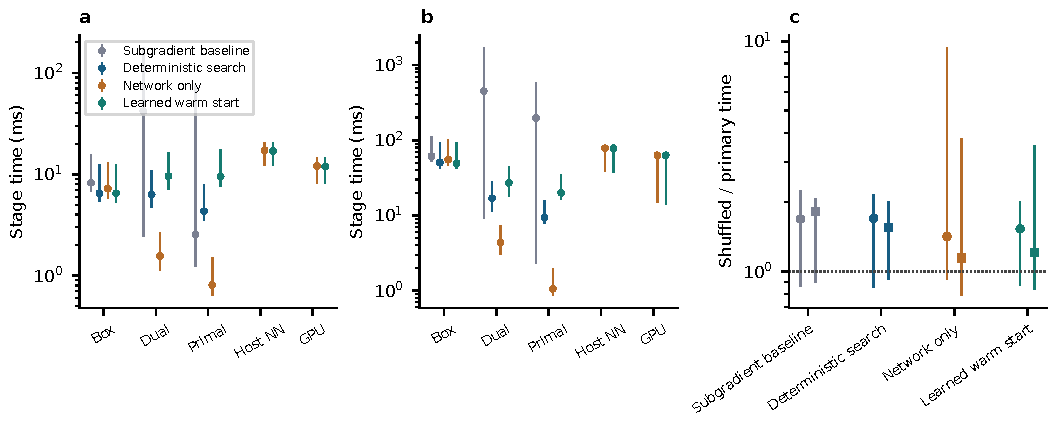
\includegraphics[width=\linewidth]{supplementary/figures/sfig4.pdf}
\caption{Stage-time and load sensitivity. Panels a and b show 32 and 64 users, respectively; panel c shows the shuffled-order comparison. Left and centre, dots show medians and whiskers show p05--p95 across 512 block-level stage medians. Zero GPU/host-network times for the classical methods are omitted on the log axis. GPU and host neural intervals overlap. Right, p05/median/p95 of shuffled-call latency divided by the same block's original median, for 52 blocks. Circles denote 32 users and squares 64 users. Colours identify the same methods throughout.}\label{supp:fig2}
\end{figure}
